\documentclass{jsarticle}
\usepackage{amsmath,amssymb}
\usepackage[dvipdfmx]{graphicx}

\usepackage{tikz}
\usepackage{circuitikz}
\usetikzlibrary{arrows,shapes.gates.logic.US,shapes.gates.logic.IEC,calc}
\begin{document}


%以下FF
\tikzset{ff/.style={flipflop, flipflop def={
  t1={D}, t2={}, c3=1, t4={},t5={},t6={Q},clock wedge size=.3, nd=0}},
}


\begin{figure}[h]
  \begin{center}
    \begin{tikzpicture}
      \node[ff](FF1){FF};
      \node[not gate US, draw, rotate=180] at ($(FF1.pin 1)!0.5!(FF1.pin 6)+(0,1)$) (Not) {};
      \draw (FF1.pin 1) -- ++ (-0.15,0)
      to[short]++(0,1);
      \draw (FF1.pin 6) -- ++ (0.15,0)
      to[short]++(0,1)
      to[short](Not.input);
      \draw (Not.output)
      to[short]($(FF1.pin 1) + (-0.15,1)$);
      \draw($(FF1.down)$)
      to[short,a=rst]++(0,-0.1);
      \draw($(FF1.pin 3)$)
      to[short,a=clk]++(-0.15,0);
      \draw($(FF1.down)$)
      to[short]++(0,0.29);
    \end{tikzpicture}
  \end{center}
   \caption{flipflop}
\end{figure}

%以下Latch
\tikzset{latch/.style={flipflop, flipflop def={
  t1={D}, t2={}, t3={clk}, t4={},t5={},t6={Q}, nu=0}},
}

\begin{figure}[h]
  \begin{center}
    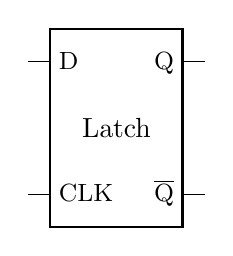
\begin{tikzpicture}
      \node[latch]{Latch};
    \end{tikzpicture}
  \end{center}
   \caption{latch}
\end{figure}



\end{document}
